%% 
%% Copyright 2007-2020 Elsevier Ltd
%% 
%% This file is part of the 'Elsarticle Bundle'.
%% ---------------------------------------------
%% 
%% It may be distributed under the conditions of the LaTeX Project Public
%% License, either version 1.2 of this license or (at your option) any
%% later version.  The latest version of this license is in
%%    http://www.latex-project.org/lppl.txt
%% and version 1.2 or later is part of all distributions of LaTeX
%% version 1999/12/01 or later.
%% 
%% The list of all files belonging to the 'Elsarticle Bundle' is
%% given in the file `manifest.txt'.
%% 
%% Template article for Elsevier's document class `elsarticle'
%% with harvard style bibliographic references

\documentclass[preprint,12pt]{elsarticle}
%\documentclass[final,5p,times,twocolumn]{elsarticle} 
% Adapt figure at about line 887 when documentclass is changed

% Suppress display of footer ``Submitted to ...'', see https://tex.stackexchange.com/questions/35712/modify-footer-used-by-elsarticle-cls
\makeatletter
\def\ps@pprintTitle{%
 \let\@oddhead\@empty
 \let\@evenhead\@empty
 \def\@oddfoot{\centerline{\thepage}}%
 \let\@evenfoot\@oddfoot}
\makeatother

%% Use the option review to obtain double line spacing
%% \documentclass[authoryear,preprint,review,12pt]{elsarticle}

%% Use the options 1p,twocolumn; 3p; 3p,twocolumn; 5p; or 5p,twocolumn
%% for a journal layout:
%% \documentclass[final,1p,times,authoryear]{elsarticle}
%% \documentclass[final,1p,times,twocolumn,authoryear]{elsarticle}
%% \documentclass[final,3p,times,authoryear]{elsarticle}
%% \documentclass[final,3p,times,twocolumn,authoryear]{elsarticle}
%% \documentclass[final,5p,times,authoryear]{elsarticle}
%% \documentclass[final,5p,times,twocolumn,authoryear]{elsarticle}

%% For including figures, graphicx.sty has been loaded in
%% elsarticle.cls. If you prefer to use the old commands
%% please give \usepackage{epsfig}

%% The amssymb package provides various useful mathematical symbols
\usepackage{amssymb}
%% The amsthm package provides extended theorem environments
%% \usepackage{amsthm}

%% The lineno packages adds line numbers. Start line numbering with
%% \begin{linenumbers}, end it with \end{linenumbers}. Or switch it on
%% for the whole article with \linenumbers.
%% \usepackage{lineno}

% To be able to enter URL with breaks:
\usepackage[hyphens]{url}
\usepackage{hyperref}
\usepackage{framed}

\sloppy % See anser in https://tex.stackexchange.com/questions/9107/how-can-i-make-my-text-never-go-over-the-right-margin-by-always-hyphenating-or-b  -  This prevents that SAP2Moose or Moose2Model overlap sometimes the right border.


\newdefinition{definition}{Definition}


\journal{Information and Software Technology}

\begin{document}

\begin{frontmatter}

%% Title, authors and addresses

%% use the tnoteref command within \title for footnotes;
%% use the tnotetext command for theassociated footnote;
%% use the fnref command within \author or \affiliation for footnotes;
%% use the fntext command for theassociated footnote;
%% use the corref command within \author for corresponding author footnotes;
%% use the cortext command for theassociated footnote;
%% use the ead command for the email address,
%% and the form \ead[url] for the home page:
%% \title{Title\tnoteref{label1}}
%% \tnotetext[label1]{}
%% \author{Name\corref{cor1}\fnref{label2}}
%% \ead{email address}
%% \ead[url]{home page}
%% \fntext[label2]{}
%% \cortext[cor1]{}
%% \affiliation{organization={},
%%            addressline={}, 
%%            city={},
%%            postcode={}, 
%%            state={},
%%            country={}}
%% \fntext[label3]{}

\title{The SOMIX Metamodel}

%% use optional labels to link authors explicitly to addresses:
%% \author[label1,label2]{}
%% \affiliation[label1]{organization={},
%%             addressline={},
%%             city={},
%%             postcode={},
%%             state={},
%%             country={}}
%%
%% \affiliation[label2]{organization={},
%%             addressline={},
%%             city={},
%%             postcode={},
%%             state={},
%%             country={}}

\author[1]{Rainer Wolfgang Winkler\corref{cor1}%
%\fnref{fn1}
}
\ead{rainer.winkler@cubeserv.com}
\address[1]{CubeServ GmbH, Am Prime-Parc 4, 65479 Raunheim, Germany}

\cortext[cor1]{Corresponding author}

%\author{Rainer Wolfgang Winkler}
%\adress{Test}
%\affiliation{organization={CubeServ GmbH},%Department and Organization
%            addressline={Am Prime-Parc 4}, 
%            city={Raunheim},
%            postcode={65479}, 
%%            state={},
%            country={Germany}}

\begin{abstract}

The SOMIX Metamodel is specified.

\end{abstract}


\begin{keyword}
% Up to 6 keywords in british spelling. Avoid general and plural terms.
%% keywords here, in the form: keyword \sep keyword

%Program Comprehension \sep
Software exploration \sep
%Code Comprehension \sep
Software maintenance \sep
Software visualization \sep
SAP development

%% PACS codes here, in the form: \PACS code \sep code

%% MSC codes here, in the form: \MSC code \sep code
%% or \MSC[2008] code \sep code (2000 is the default)

\end{keyword}

\end{frontmatter}

%% \linenumbers

%%%%%%%%%%%%%%%%%%%%%%%%%%%%%%%%%%%%%%%%%%%%%%%%%%%%%%
\section{Introduction}
\label{intro}
The SOMIX Metamodel is specified in a similar way as FAMIX~\cite{r_Ducasse_2011}.
This metamodel is a concrete specification of a type of metamodel described in~\cite{r_Metamodel_Preprint_2}.
Such a metamodel can be read and displayed by the JavaScript version~\cite{r_Moose2Model2} of Moose2Model~\cite{r_Moose2Model}. The extraction tool SAP2Moose~\cite{r_SAP2Moose} provides currently models in the SOMIX format.

\section{Software Metamodel}
\subsection{Overview of SOMIX}


\begin{figure} [h!] 
\centering

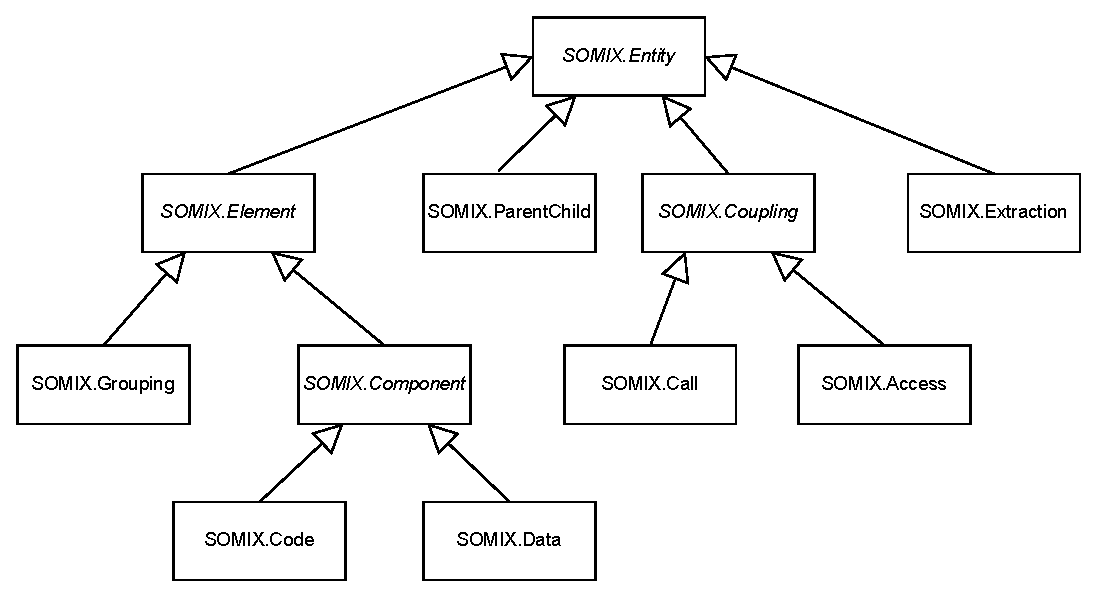
\includegraphics[width=1\columnwidth]{SOMIX_Classes.inkscape.eps} 
\caption{
The classes of the SOMIX Metamodel
}
\label{fig:InterfaceExample}   
\end{figure}
\subsection{Classes}

\subsubsection{SOMIX.Entity}

SOMIX.Entity is the abstract root class of the SOMIX metamodel entities.

Fields:
\begin{itemize}
\item In SAP2Moose: The mse model where it is contained.
\end{itemize}


\subsubsection{SOMIX.Element extends SOMIX.Entity}

SOMIX.Element is the abstract super class for all components or groupings in a software.

Fields:
\begin{itemize}
\item name: A mandatory string with the name of the grouping or component in the system.
\item uniqueName: A mandatory unique string with the name of the grouping or component in the system.\\
It has to be the same for all extractors which extract a certain element. When this is not the case a mapping has to be provided to support matching elements.\\
uniqueName is always in lower case when the names are not case sensitive in the extracted system.\\
The combination of technicalType and uniqueName determines an element completly.
\item title: An optional string with the title of the grouping or component in the system.
\item technicalType: A string with information about the kind of grouping or component.
\item linkToEditor: A link to open the specified element in an editor.
\end{itemize}



\subsubsection{SOMIX.Grouping extends SOMIX.Element}

SOMIX.Grouping is used for all parts of a system that group other parts.

\subsubsection{SOMIX.Component extends SOMIX.Element}

SOMIX.Component is the abstract super class for code and data.

Fields:
\begin{itemize}
\item isPartOf: Optional: When the component is part of another component: The instance of SOMIX.Component it is a part of. When the instance is of type SOMIX.Code this has also to be an instance of SOMIX.Code. When the instance is of type SOMIX.Data this has also to be an instance of SOMIX.Data.
\item partSpecification: When isPartOf is set: A string where the kind of part is specified.
\end{itemize}

\subsubsection{SOMIX.Code extends SOMIX.Component}

SOMIX.Code is used for all components of a system that have logic.

\subsubsection{SOMIX.Data extends SOMIX.Component}

SOMIX.Data is used for all components of a system that have no logic. This is normally data or a view on data.

Fields:
\begin{itemize}
\item isPersistent: Set to true to mark that data is stored persistently. This allows it to mark database table visually in a system.
\end{itemize}

\subsubsection{SOMIX.ParentChild extends SOMIX.Entity}

SOMIX.ParentChild is used to specify parent-child relations.

Fields:
\begin{itemize}
\item parent: An instance of SOMIX.Grouping.
\item child: An instance of SOMIX.Element or SOMIX.Grouping.
\item isMain: A boolean that the parent child relation should be shown always in a diagram. Only a single parent of a child should be flagged like this. Diagram tools should display the parent of a child always when this flag is set. This assures for instance that a class is always displayed when an attribute or method of a class is displayed in a diagram.
\end{itemize}


\subsubsection{SOMIX.Coupling extends SOMIX.Entity}

SOMIX.Coupling is the abstract super class of SOMIX.Call and SOMIX.Access.

\subsubsection{SOMIX.Call extends SOMIX.Coupling}

SOMIX.Call is used to specify calls of code by other code.

Fields:
\begin{itemize}
\item caller: An instance of SOMIX.Code.
\item called: An instance of SOMIX.Code.
\end{itemize}

\subsubsection{SOMIX.Access extends SOMIX.Coupling}
SOMIX.Access is used to specify read or write accesses. When all three flags isWrite, isRead, and isDependent are false, the Access has to be regarded as not existing by an analyzing application. When multiple Accesses exists for the same combination of components an analyzing application has to combine this into a single access. The fields isWrite, isRead, and isDependent are true when they are true in at least one of the combined accesses.

Fields:
\begin{itemize}
\item accessor: An instance of SOMIX.Component.
\item accessed: An instance of SOMIX.Data.
\item isWrite: A flag whether a write access is made or might be made.
\item isRead: A flag whether a read access is made or might be made. 
\item isDependent: A flag whether a further dependency exists or might exist.
\end{itemize}



\subsubsection{SOMIX.Extraction extends SOMIX.Entity}
Contains fields with metadata of the extraction. This is mandatory because the mse model itself contains no metadata. It is proposed in Ducasse et al. to store metadata as part of the model~\cite{r_Ducasse_2011}.

Fields:
\begin{itemize}
\item extractionTime: The date, time and timezone when the extraction was started.
\item system: A string with the name of the extracted system.
\end{itemize}


\section*{Declaration of Competing Interests} 
The author declares that he has no known competing financial interests or personal relationships that could have appeared to influence the work reported in this paper.

\section*{Acknowledgments}

This work was funded by CubeServ GmbH.
Many colleagues provided valuable support to make this project possible.
I thank
Patrick Michels for providing resources and support.



\begin{thebibliography}{00}
\bibitem{r_Ducasse_2011}
S. Ducasse, N. Anquetil, M.U. Bhatti, A.C. Hora, J. Laval, T. Girba, MSE and FAMIX 3.0: An Interexchange Format and Source Code Model Family. Research Report, Nov 2011. [Online], available: \url{https://hal.inria.fr/hal-00646884}.
\bibitem{r_Metamodel_Preprint_2}
Winkler, Rainer Wolfgang, A Software Metamodel Restricted to Key Aspects of a Software System for Developers and a Method to Keep Manually Drawn Diagrams Up-to-Date and Correct. Available at SSRN: https://ssrn.com/abstract=4049604 or http://dx.doi.org/10.2139/ssrn.4049604.
\bibitem{r_Moose2Model2}
Moose2Model, \url{https://github.com/Moose2Model/Moose2Model2} (accessed 12 September 2022).
\bibitem{r_Moose2Model}
Moose2Model, \url{https://github.com/Moose2Model/Moose2Model} (accessed 30 December 2020).
\bibitem{r_SAP2Moose}
SAP2Moose, \url{https://github.com/SAP2Moose/SAP2Moose} (accessed 30 December 2020).

\end{thebibliography}
\end{document}

\endinput
%%
%% End of file `elsarticle-template-harv.tex'.
